% DESENVOLVIMENTO DA APLICAÇÃO-------------------------------------------------------------------

\chapter{DESENVOLVIMENTO DA APLICAÇÃO}
A proposta para este trabalho foi a construção de uma API que ficaria responsável
por aguardar e coletar as coordenadas geográficas dos pedidos gerados no estabelecimento,
juntamente com o desenvolvimento de uma aplicação encarregada de gerenciar os pedidos como entregas
com um painel de controle para geração de lotes de entregas e o desenvolvimento de um módulo destinado ao motoboy, no qual consegue observar, em um mapa, a rota e pontos de parada que devem ser percorridos no lote disponível para entrega, tudo isso em tempo real.

\section{Softwares utilizados}
Esta Seção apresenta os \textit{softwares} utilizados na etapa de codificação da aplicação.

\begin{itemize}
    \item PhpStorm: IDE completa de desenvolvimento para projetos codificados com a linguagem de programação PHP;
    \item Composer: gerenciador de pacotes em nível de aplicativo, que fornece um formato padrão para gerenciar dependências de software PHP e bibliotecas necessárias;
    \item Cmder: console para execução de linhas de comandos para o sistema operacional Windows, com essa ferramenta é possível executar comandos Unix (\textit{ls}, \textit{rm}, \textit{mv} e etc) diretamente no Windows;
    \item Laravel: \textit{framework} de programação baseada na linguagem PHP;
    \item Artisan CLI: interface de linha de comando incluída no Laravel, fornecendo vários comandos úteis durante a criação da aplicação, por exemplo: configuração de ambiente, verificar rotas, interagir com a aplicação e criar diversos tipos de arquivos (\textit{Migrations}, \textit{Controllers} e \textit{Models});
    \item Blade: ferramenta para criação de interface gráfica, utilizado pelo Laravel como uma ferramenta de \textit{template}, trazendo uma quantidade grande de funcionalidades que ajudam na criação de interfaces interativas;
    \item Eloquent ORM: ferramenta com funcionalidades que facilitam a inserção, atualização, busca e exclusão de registros diretamente no banco de dados;
    \item XAMPP: servidor independente de plataforma, que inclui: Apache, MySQL, phpMyAdmin, FileZilla FTP Server, OpenSSL, PHP e Perl;
    \item Jaspersoft Studio: ferramenta para projetar e executar modelos de relatório com  expressões, gráficos, mapas, tabelas e \textit{QR Codes}, criando documentos de qualquer complexidade a partir de informações presentes no banco de dados;
    \item GitHub: plataforma de hospedagem de código-fonte com controle de versão;
    \item Sourcetree: representação visual de repositórios da nuvem.
\end{itemize}

\newpage
Para desenvolvimento do servidor deste trabalho, foi escolhido trabalhar com Laravel, um \textit{framework} baseado na linguagem PHP de programação, em conjunto com o XAMPP, um servidor independente de plataforma para rodar sistemas localmente, que consiste principalmente na base de dados MySQL, o servidor web Apache e os interpretadores para linguagens de \textit{script}: PHP e Perl, o que facilita e agiliza o desenvolvimento. Como o conteúdo estará armazenado numa rede local, o acesso aos arquivos é realizado instantaneamente, ficando disponível no endereço \textit{http://127.0.0.1}.

Ao utilizar o comando \textit{composer create-project --prefer-dist laravel/laravel delivery-routes} no Cmder, dentro de uma pasta no sistema operacional destinada a programação da aplicação, foi criada a estrutura base do projeto, cedida pelo Laravel, apresentada na \autoref{fig:base-projeto}. A facilidade na criação do projeto se deve ao Cmder, que torna o trabalho no sistema operacional da Microsoft mais agradável, com essa ferramenta é possível rodar comandos do Linux e MAC que são baseados em Unix para o Windows. 

\begin{figure}[H]
    \centering
    \caption{Estrutura Laravel}
    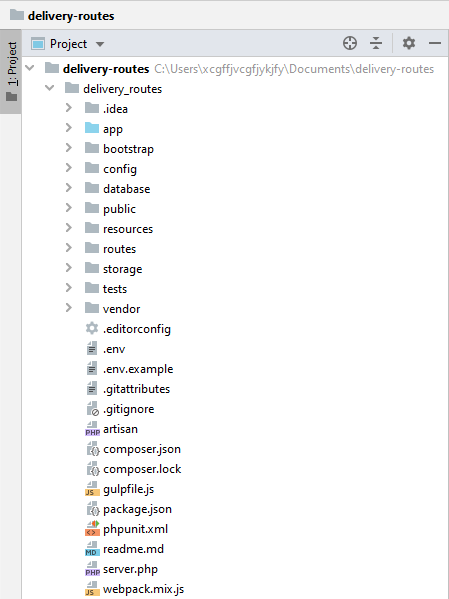
\includegraphics[width=0.6\textwidth]{./dados/figuras/fig6}
    \fonte{Autor}
    \label{fig:base-projeto}
\end{figure}

\newpage
Foi necessária uma série de configurações de ambiente para que se tornasse possível o desenvolvimento da aplicação: primeiramente foi preciso instalar e configurar todas as dependências do PHP para que se pudesse ter acesso a linguagem de programação através do gerenciados de dependências Composer. Esta etapa contou com o auxílio do Cmder, terminal para Windows que reconhece comandos Unix e do Artisan, interface de linha de comando incluída no Laravel.

Foi optado, por questões de segurança, hospedar o código-fonte do projeto em nuvem, através da plataforma GitHub. A sincronia entre os arquivos locais e o GitHub foi possível com o auxílio do sistema de controle de versões chamado Git, representado visualmente pelo Sourcetree, que deixa o trabalho braçal por linha de comando (\textit{gitbash}) de lado, sendo também necessário sua instalação e configuração na máquina de desenvolvimento. 

O banco de dados escolhido para armazenar os registros foi o MySQL cuja instalação e configuração ocorreu automaticamente pelo XAMPP, que também é responsável pela instalação do servidor web local Apache. Por último, para ter acesso a manipulação do código, um editor de texto era necessário, optando-se pelo PHPStorm, uma IDE paga, mas estudantes podem conseguir licença estudantil, terminando assim a fase configuração de ambiente de desenvolvimento e garantindo aptidão para começar os trabalhos.

O próximo passo foi a modelagem dos dados, onde verificou-se que seria necessário a criação das tabelas: \textit{users}, \textit{motoboys}, \textit{deliveries}, \textit{payments} e \textit{orders}. Uma sexta tabela chamada de \textit{deliveries\_orders} precisou ser criada para vincular mais de um pedido à cada entrega, onde uma \textit{trigger}, disparada \textit{after update}, ficou responsável pela atualização do status de cada pedido vinculado à entrega, esta chamada de \textit{tr\_Status\_Orders}, apresentada na \autoref{fig:trigger}.

\begin{figure}[H]
    \centering
    \caption{Trigger tr\_Status\_Orders}
    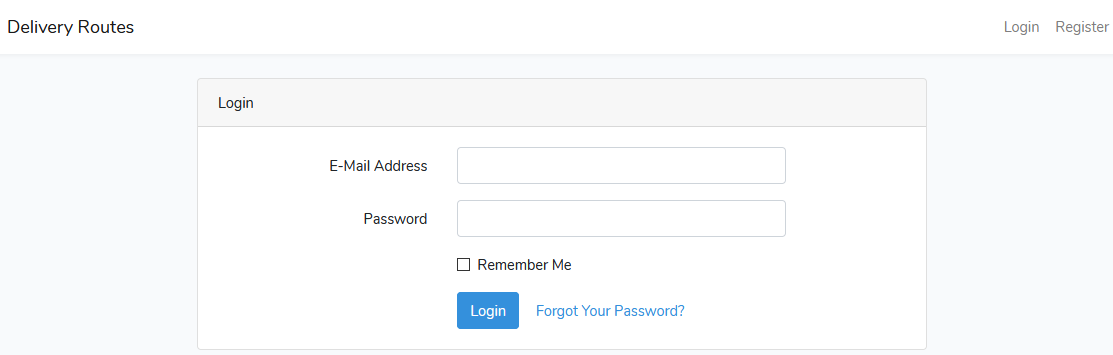
\includegraphics[width=0.7\textwidth]{./dados/figuras/fig7}
    \fonte{Autor}
    \label{fig:trigger}
\end{figure}

%\begin{algorithm}[H]
 
\section{Coleta de dados}

\section{Módulo de gerenciamento}
%%% Rev-Madalozzo: Aqui no módulo de gerenciamento sugiro você listar todos os pacotes de terceiros que é util e que você utilizou na tua aplicação. Por exemplo, na aula usamos o AdminLTE e PDF, caso tu uso algum módulo de terceiros lista neste Capítulo 

\section{Consulta de dados}

\section{Módulo de entrega}

%Figura 29 - Trecho de código em PHP para calcular a proporção de cada cluster no contexto do usuário
%O trecho de código fonte que é apresentado a seguir demonstra como é o serviço de                login do aplicativo: 
%, conforme apresenta a figura 19 
%, conforme a figura 20 mostra
%\caption{Delivery Routes - Página inicial}